In this section we present and comment on our results from simulations of the three different models. Wealth distribution diagrams show the distribution of agents with respect to how much money they have. In most wealth distribution diagrams we also show the correlation of the data to various analytically known distributions, some of which are familiar and well studied, like Gibbs (Boltzmann) and Pareto. 
All simulations have a uniform distribution of wealth among the agents, where $m_0 = 1$, as the initial state.
For the results to be representative it is important to have enough transactions to allow for the system to settle at some equilibrium. Such a macrostate is reached when the systems overall distribution does not change even if we perform many more transactions. The results are all controlled for this empirically by studying the evolution of the distribution through a range of montecarlo cycles (representing the time dependence of the system).

\begin{figure}[H]
    \centering
    \begin{subfigure}{0.5\textwidth}
        \centering
        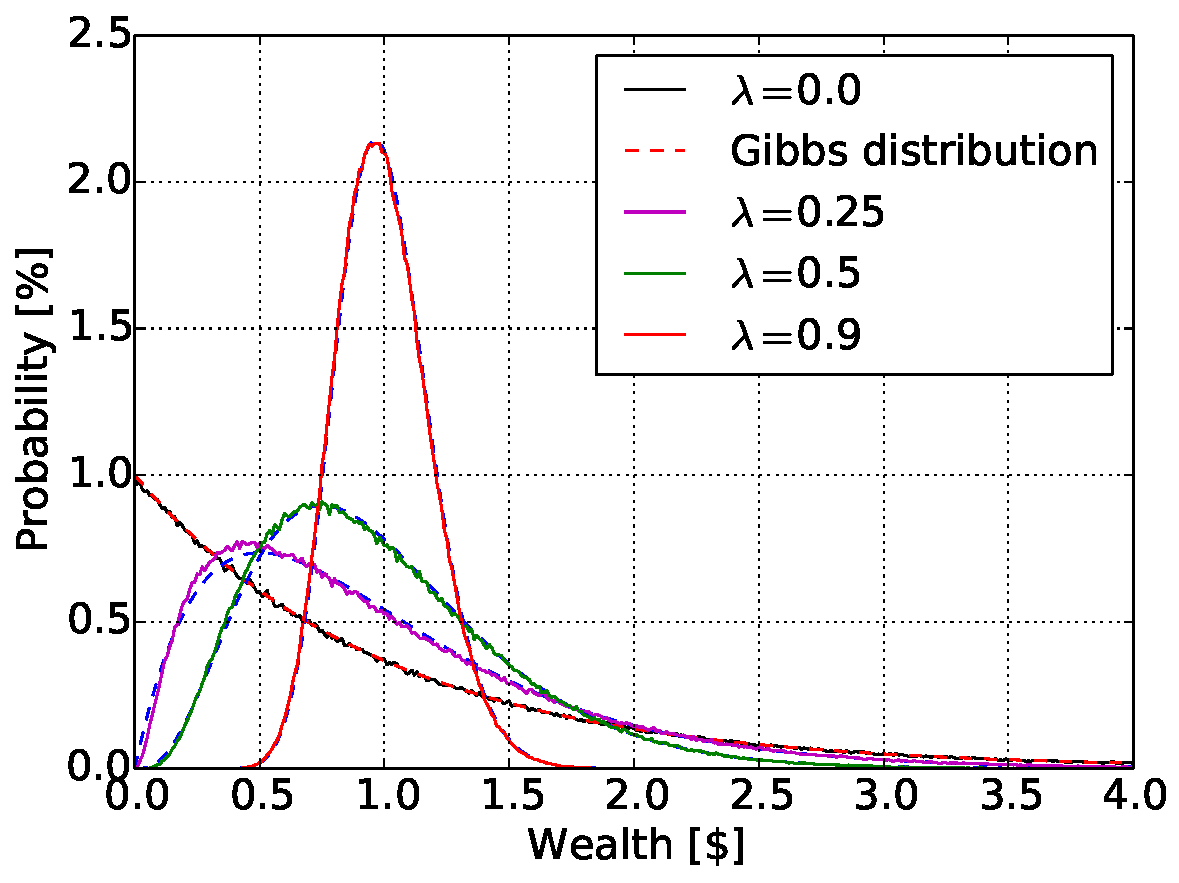
\includegraphics[width=\linewidth]{result/bilder/5c}
        \caption{}
        \label{fig:wealthForLambda}
    \end{subfigure}%
    ~ 
    \begin{subfigure}{0.5\textwidth}
        \centering
        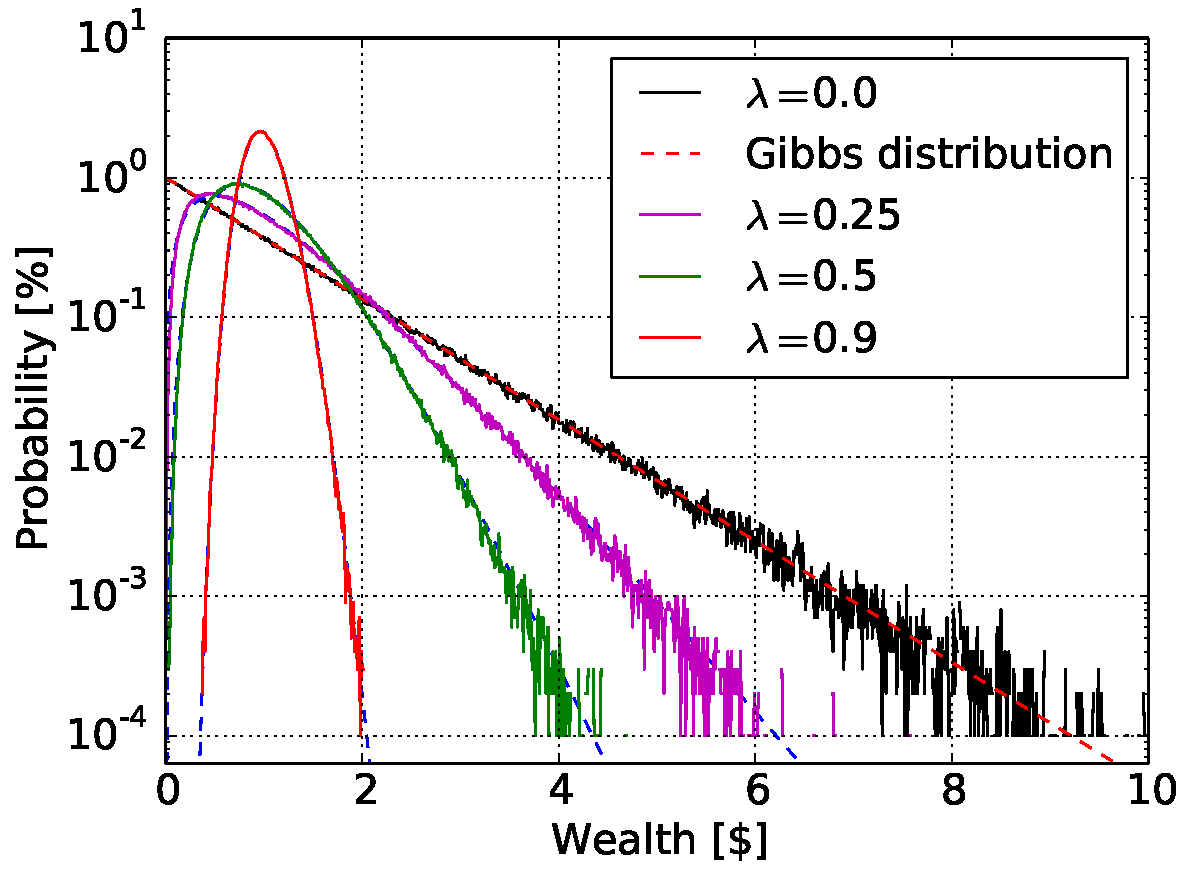
\includegraphics[width=\linewidth]{result/bilder/5c-log}
        \caption{}
        \label{fig:wealthForLambdaLog}
    \end{subfigure}
    \caption{a) shows how the agents are distributed with respect to their wealth. b) log plot of the case where $\lambda = 0$}
\end{figure}

Figure \ref{fig:wealthForLambda} shows how the distribution changes depending on the savings parameter $\lambda$ (which is equal for all agents). When the agents always allow for their entire wealth to be part of a transaction we get a gibbs distribution. We see that a few agents are very wealthy compared to the majority who are rather poor. When the agents are allowed to save a certain amount of their wealth (i.e. exclude a fraction of their wealth from taking part of a transaction) there are both major and minor changes to the wealth distribution. The most striking feature being the reduction in number of very poor agents, even at low savings. The chance of loosing even more money if you are alrady poor is diminished if you save some of your money before agreeing to a transaction. At the other end of the scale we see that only a large $\lambda$ will influence the distribution of very wealthy agents. As the saving parameter is increased further a peak is introduced to the distribution. As $\lambda\rightarrow 1$ the position of this peak approaches one (the average wealth). The deviation in the distribution from this peak is also narrowed. For the extreme case where $\lambda=1$ no money is allowed to be part of transactions so the system remains in the initial state where every agent is equally wealthy. A fitting of these curves as given in the paper by Patricia et.al. \cite{patriarca} was found to be reproducable in our results. This function is given by the equation 

\begin{equation}
    P_n(x)=a_nx^{n-1}\exp{-nx}
    \label{eq:patFit}
\end{equation}
Where
\begin{align*}
    n(\lambda)=1+\frac{3\lambda}{1-\lambda},\qquad a_n=\frac{n^n}{\Gamma(n)}
\end{align*}
 this can be found as the dashed blue line in plot \ref{fig:wealthForLambda} and correlates strongly with the associated results from our computational simulation ($\lambda$ being the same).\\


In the logarithmic plot for the same distributions, shown in figure \ref{fig:wealthForLambdaLog}, a more detailed impression of the outliers in the distribution is obtained. As shown in section 2.1 we see that the gibbs distribution is linear; and our results for the no savings case follows this trend. The $\lambda \neq 0$ distributions however are not linear, again displaying a major distinction between them. At the very high ends however they all show a linear trend (admittedly with differing slopes that still allow for wildly varying probabilities of achieving these extreme values).

\begin{figure}[H]
    \centering
    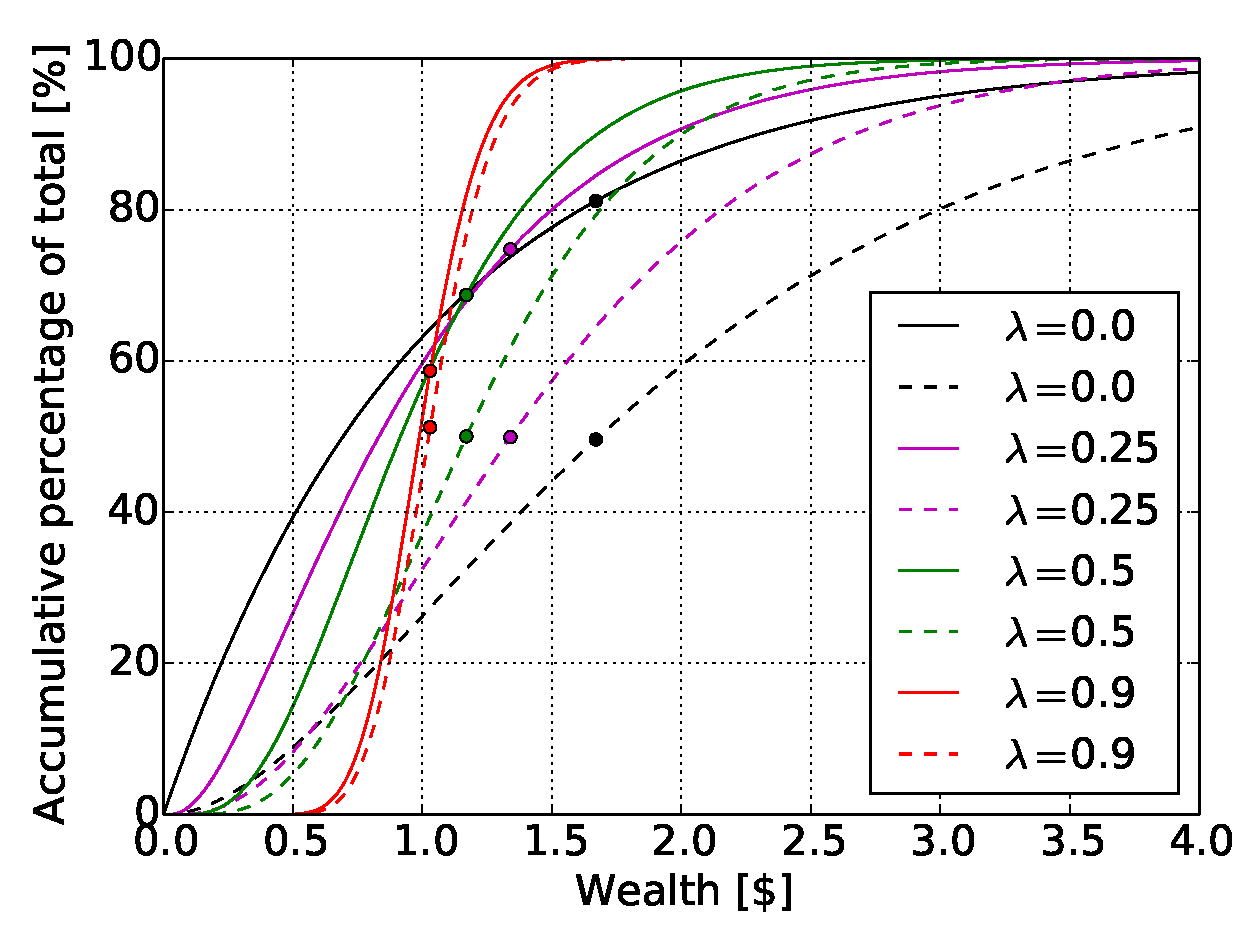
\includegraphics[width = 0.7\linewidth]{result/5c-accu-persons-accu-money}
    \caption{Accumulative percentage of total for both wealth and population. Dashed lines is for wealth, solid lines is population and dots corresponds to 50 \% of total wealth.}
    \label{fig:accu1}
\end{figure}

Figure \ref{fig:accu1} gives a more thorough picture of the wealth distribution compared to the population distribution. The y-axis gives the percentage of the total of either the wealth or the number of agents up until that point (from left to right). The plots therefore converge towards 100\% when nearing the end. Having both population and wealth in the same plot allows for a comparison of how these changes with respect to each other as you climb through the economic classes. The gap between each pair represents the disjunction between population and wealth distribution, meaning that the population up until that point does not own a fair share of the wealth. The closer the lines are to one another the more even the distribution. We see again see that this is the case for a higher value of $\lambda$, and vice versa. The slope (derivative) of the curves indicate how quickly new members are added to the total. In figure \ref{fig:accu2} is a similar plot but with respect to $\alpha$ instead of $\lambda$.\\

For the following wealth distributions we have $\alpha\neq 0$ so that there is a larger probability for people with similar amounts of money to perform transactions.
\begin{figure}[H]
    \centering
    \begin{subfigure}{0.5\textwidth}
        \centering
        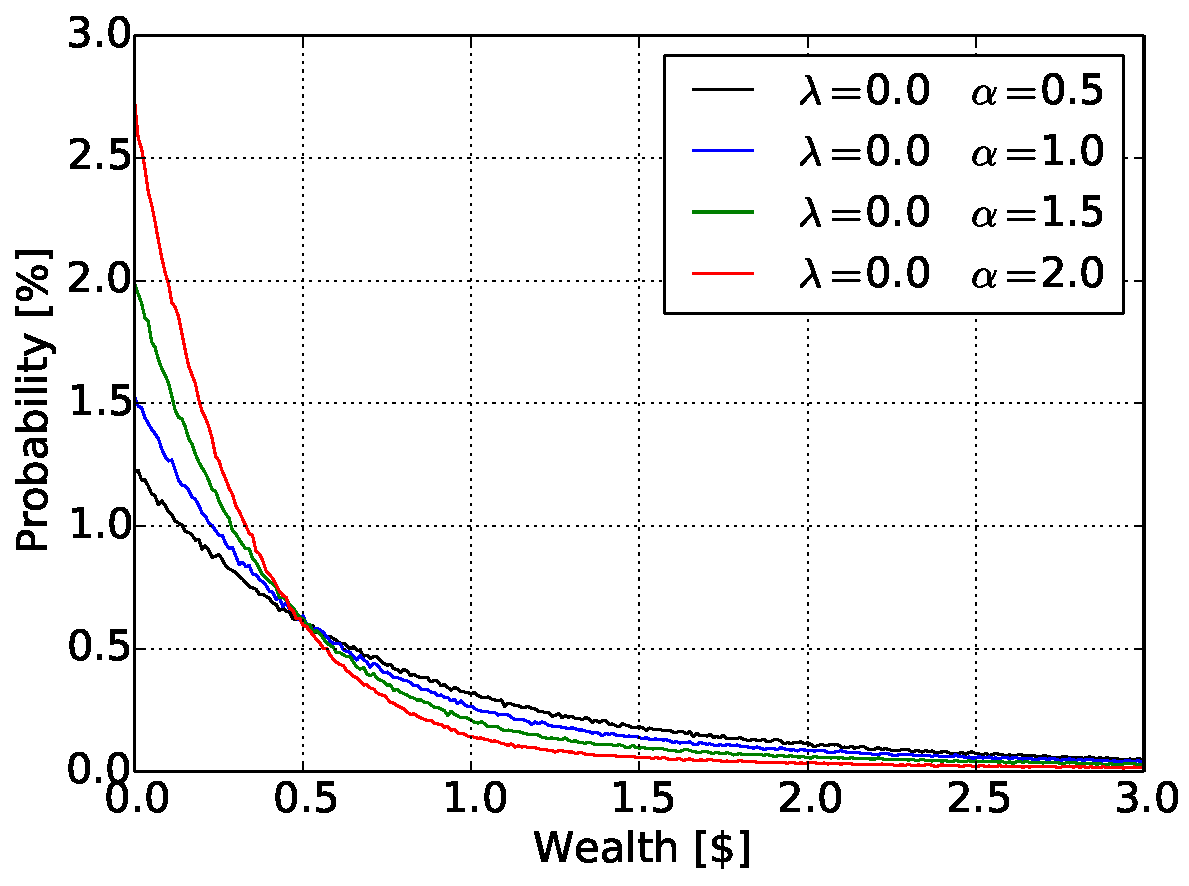
\includegraphics[width=\linewidth]{result/bilder/5d-00}
        \caption{}
    \end{subfigure}%
    ~ 
    \begin{subfigure}{0.5\textwidth}
        \centering
        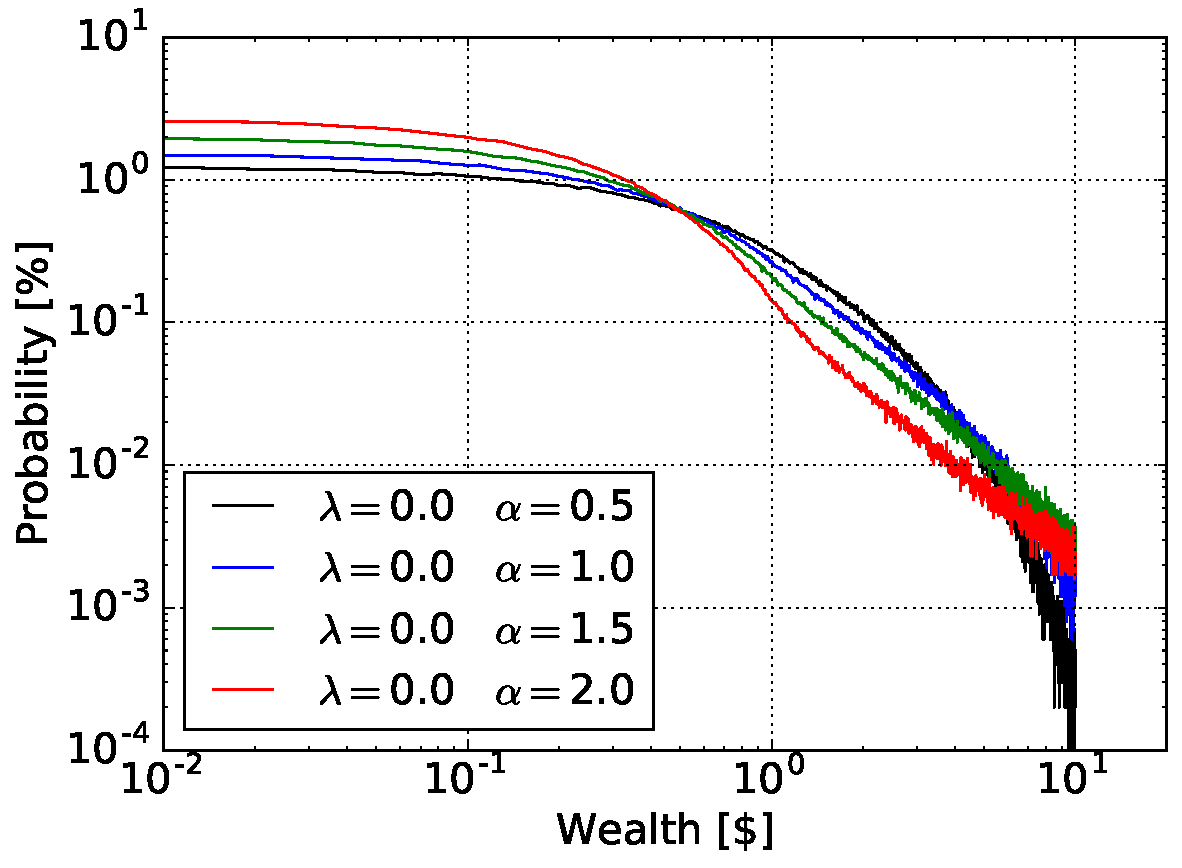
\includegraphics[width=\linewidth]{result/bilder/5d-00-loglog}
        \caption{}
    \end{subfigure}
    \caption{plots a) and b) shows the same four distributions where there is no saving and four different values for alpha. The latter is logarithmic while the former is not}
    \label{fig:5b}
\end{figure}

The trends of the graphs in figure \ref{fig:5b} clearly indicates that the new model leads to a greater difference in the low end vs the high end of the distribution. The number of poor people increases with $\alpha$ while the number of rich people decreases. Again, it is important to note that the plots represent histograms of agents and their wealth. Since there now are more poor people the sum of their wealth represents a larger amount of the total wealth than if there was a smaller population of poor people. This means, as is confirmed by summation of the data, that the money is still conserved even though there are more poor people and fewer rich people. The plots seems to intersect at around 0.5, setting the boundary at which the wealth is separated.
By studying the logarithmic plot we see that distribution lines actually intersect a second time. This means that the extremely rich actually get even richer if the population has a strong bias towards transacting with agents in their financial class. \footnote{Due to computational constraints we exclude the distribution of agents with $m_j\geq10$ which for this particular plot, unfortunately, would be of some interest. In any case it is still possible to get a decent idea of the distribution trends through the plot} \\
The linear nature of the tails of the distributions in the logarithmic plot, particularly noticeable for higher values of $\alpha$, is a strong indicator of a power law and its slope hints at the value of the exponent in this power law. Thus an increase in alpha means that the tail end of the distribution follows a power law with a smaller (less negative) exponent.\\
\begin{figure}[H]
    \centering
    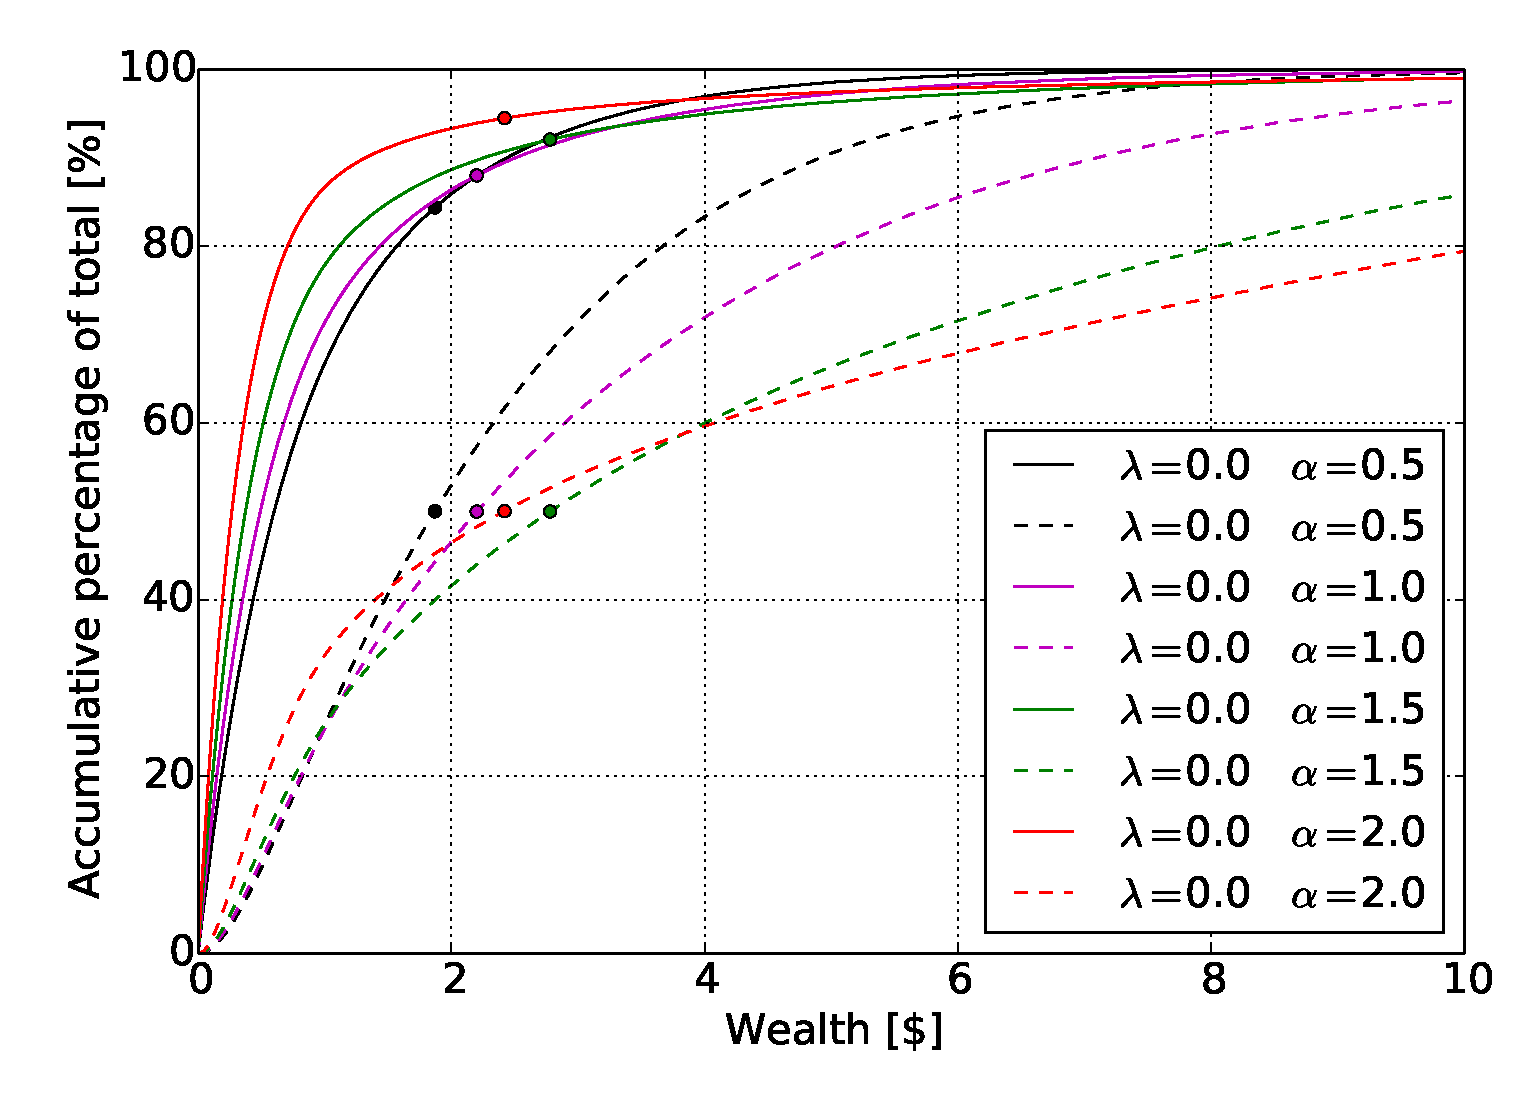
\includegraphics[width = 0.7\linewidth]{result/5d-accu-persons-accu-money}
    \caption{}
    \label{fig:accu2}
\end{figure}
Figure \ref{fig:accu2} shows the accumulative percentage the same way as was shown earlier. 
\begin{figure}[H]
    \begin{subfigure}{0.5\textwidth}
        \centering
        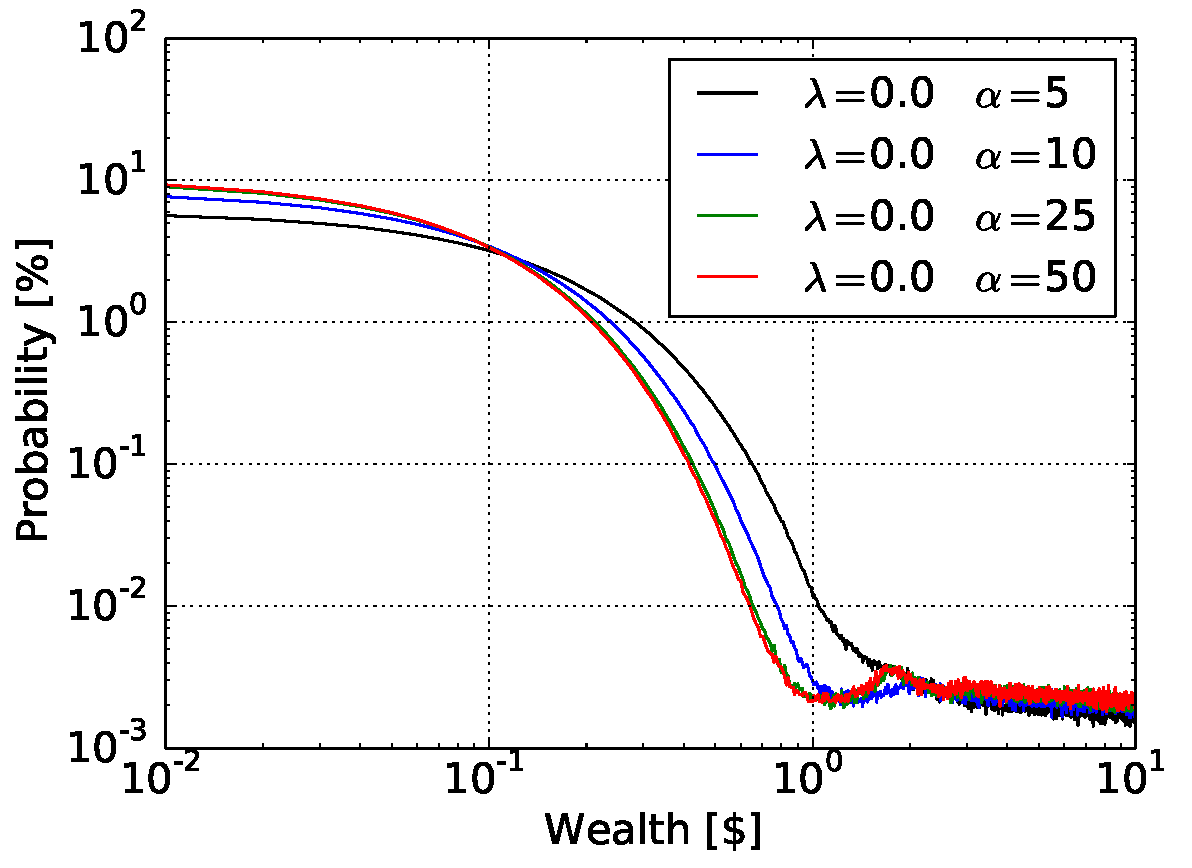
\includegraphics[width=\linewidth]{result/new_5d/5d-00-log}
        \caption{logarithmic plot wealth distribution }
        \label{fig:hugeAlpha}
    \end{subfigure}
    \begin{subfigure}{0.5\textwidth}
        \centering
        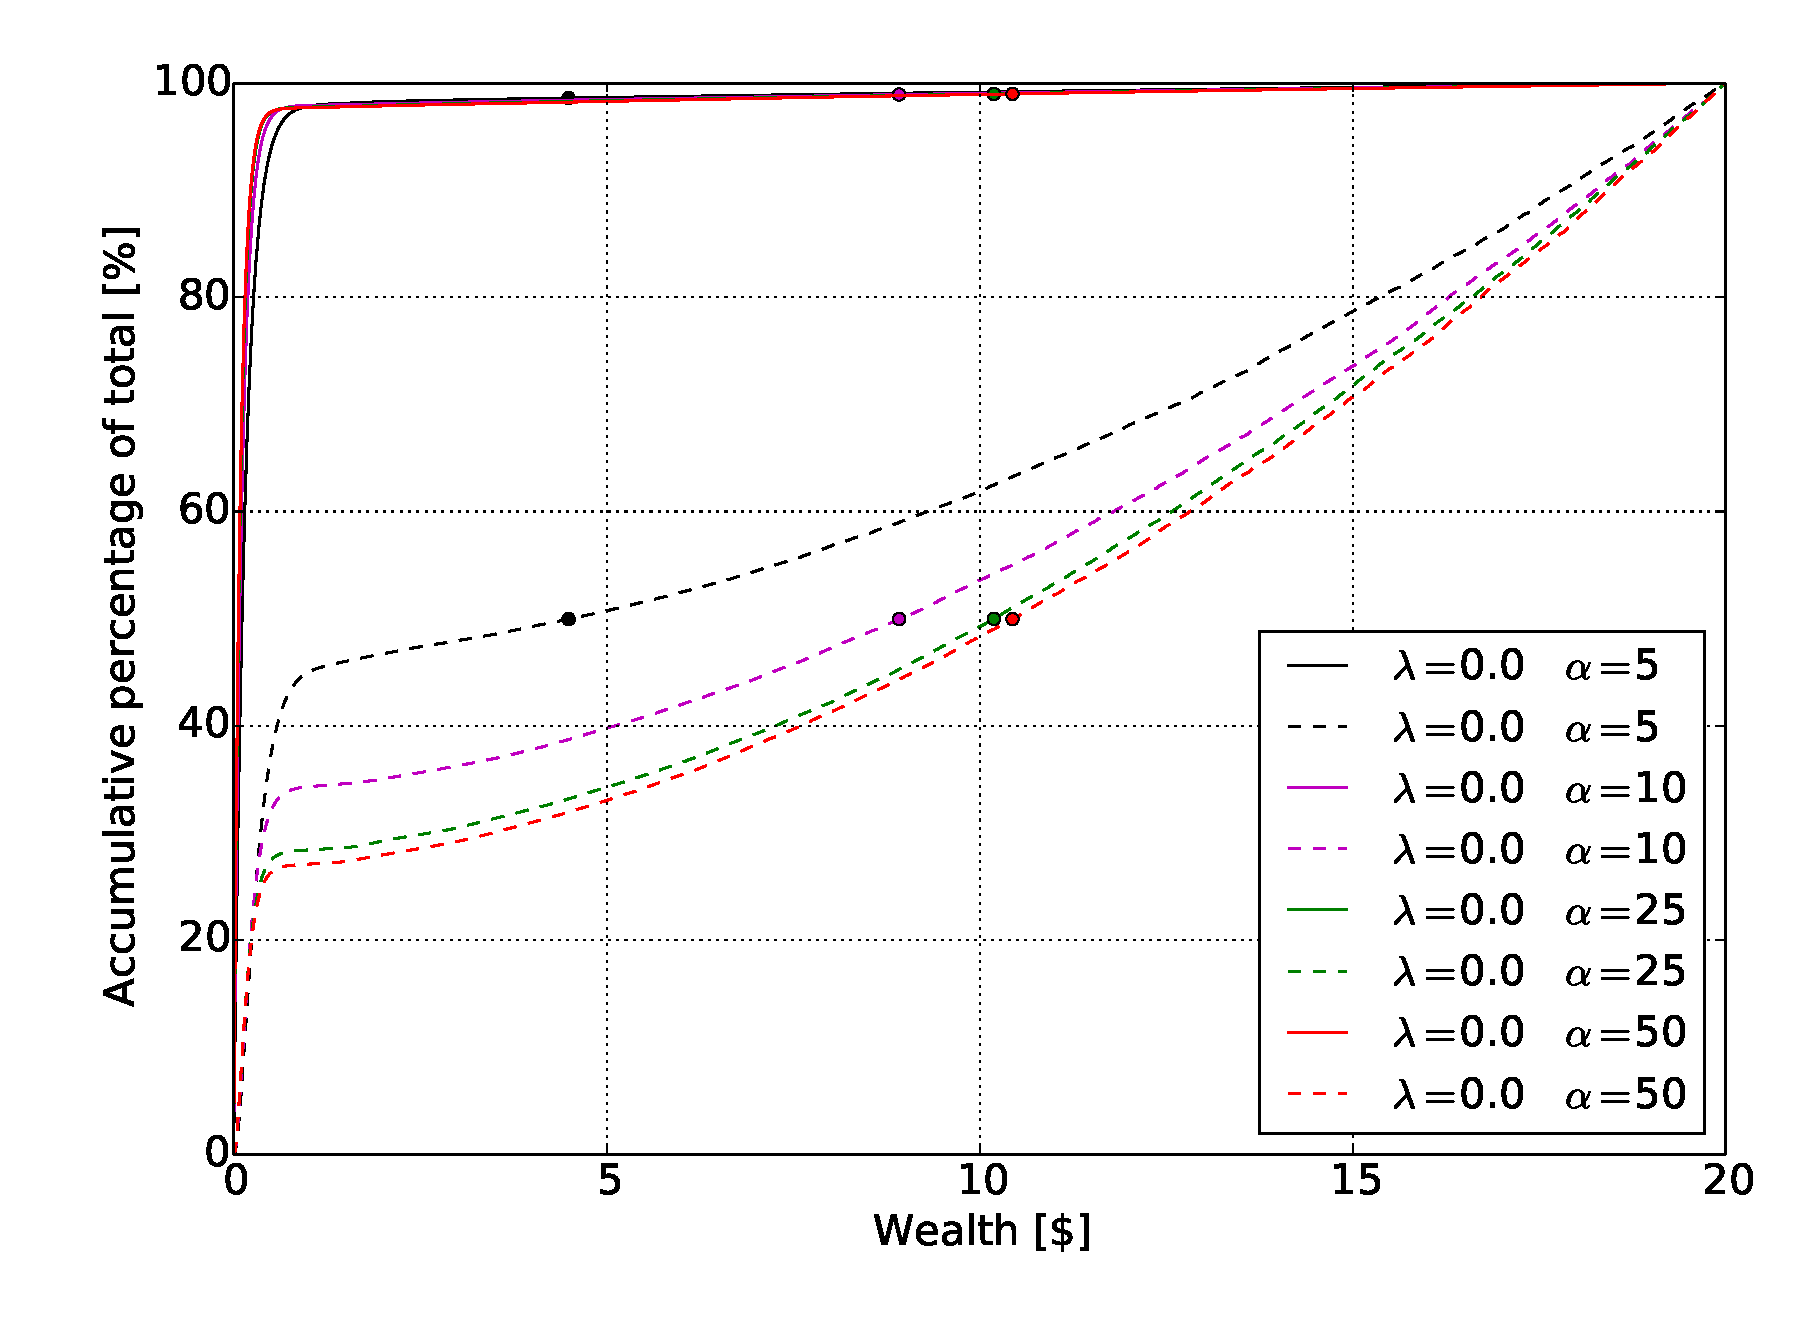
\includegraphics[width=\linewidth]{result/5d-accu-persons-accu-money-extra}
        \caption{Accumulative percentage of total for both wealth and population. Dashed line is for wealth while the others are for population}
        \label{fig:accuHugeAlpha}
    \end{subfigure}
    \caption{Plots showing trends when $\alpha >> 1$}
\end{figure}

In figure \ref{fig:hugeAlpha} we have the distributions resulting from simulations with even higher values of $\alpha$. The number of people with almost no money seems to approach 100\%. In general the curves seemingly congregate at some function limit.\\


In the plots below we combine the previous model with the new one, giving plots for different values of $\alpha$ but also $\lambda \neq 0$.
\begin{figure}[H]
    \centering
    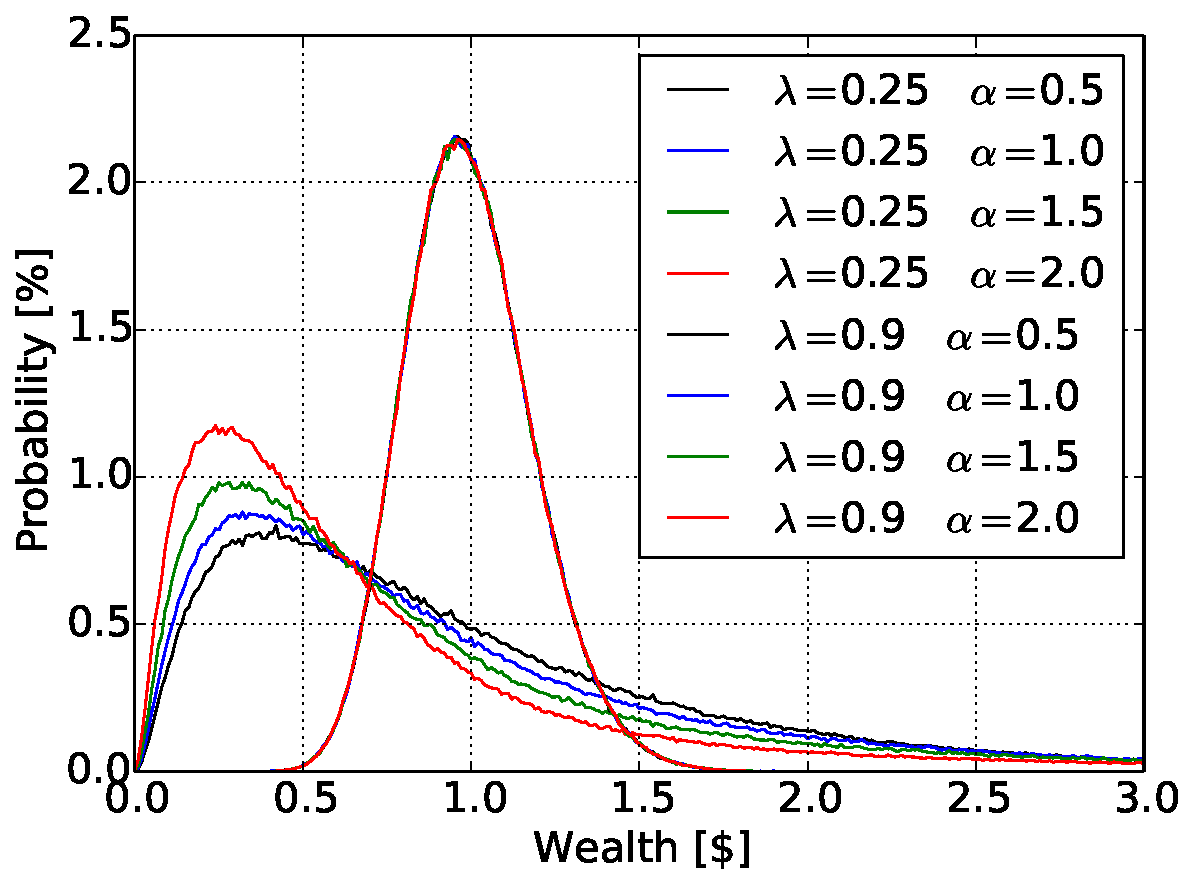
\includegraphics[width = 0.7\linewidth]{result/bilder/5d-2590}
    \caption{}
    \label{fig:5d}
\end{figure}
It seems as though the effect of agents saving money before committing to transactions has a greater impact on the distribution and dominates over the effect that preferences for same-wealth transactions has. If agents only trade using a tenth of their worth it is practically irrelevant whether they care about trading with other agents that has  a similar amount of money.\\\\

In the third model we introduce a second factor in the expression that gives the probability of having two agents follow through on an interaction. There are a total of three degrees of freedom for our system. The three parameters $\lambda$, $\alpha$ and $\gamma$ represent the weighting that's given to each of the corresponding models.

\begin{figure}[H]
    \centering
    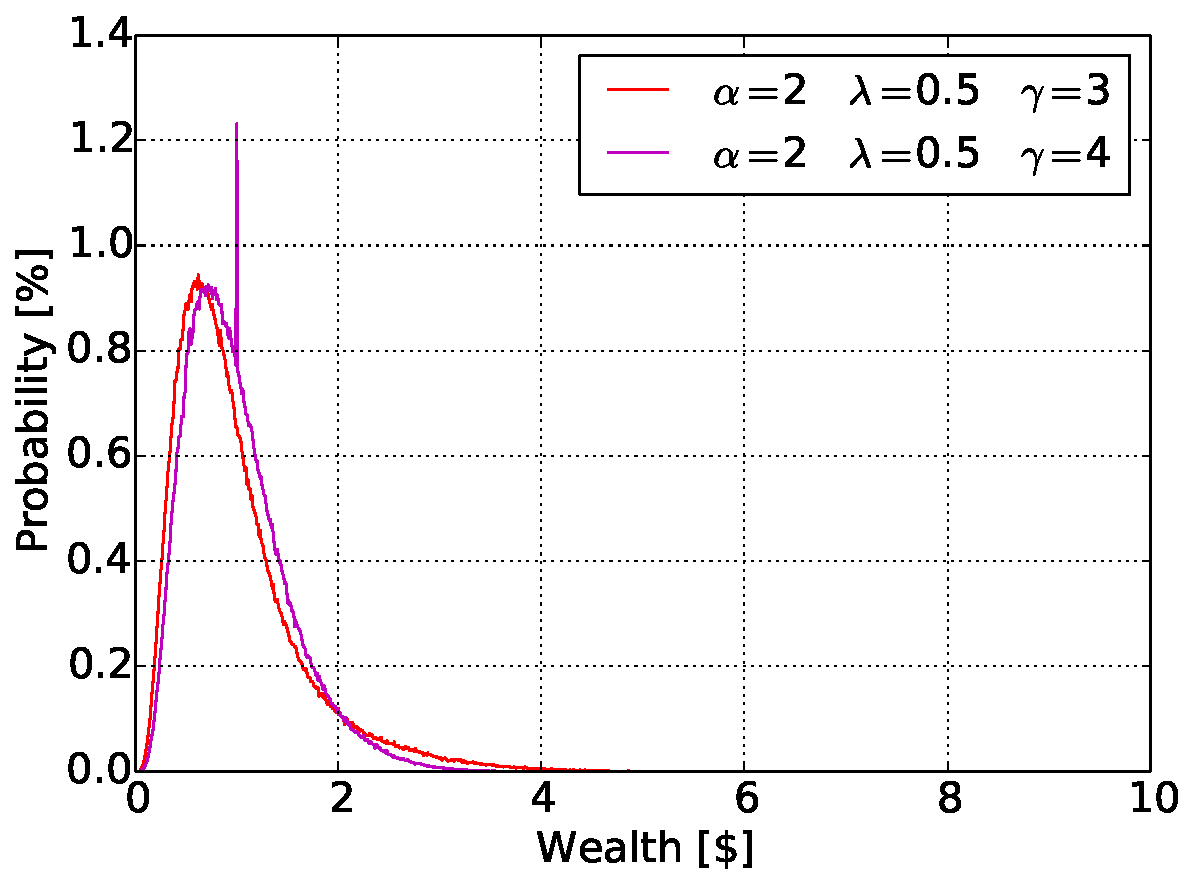
\includegraphics[width=\linewidth]{result/5e-2-50}
    \caption{wealth distribution when using the number of transactions between the two agents with the highest number of transactions for the normalization}
    \label{fig:spikeAgents}
\end{figure}

The specific implementation of the required normalization can be done in many different ways, as discussed in the normalization sections. When two agents interact and we calculate the probability for a transaction to take place we can divide the number of times they have previously traded with the number of times the most well known agents have traded (i.e. the couple who has the highest number of transactions among all agents). Figure \ref{fig:spikeAgents} illustrates how this method leaves some agents in their initial state, never trading at all. This is because the agents who are not quick enough to trade in the beginning end up with a lower chance of finding new partners to transact with; this allows other agents to trade even more which further exacerbates the situation of the lonely agents ending in a vicious cycle of ever decreasing chances of participating in the socio-economic platform of interconnected agent-relations.

We therefore choose to normalize such that each agent only consider their own transactions when determining the probability of a new transaction. All of the results are from simulations using this method. 

\begin{figure}[H]
    \centering
    \begin{subfigure}{0.5\textwidth}
        \centering
        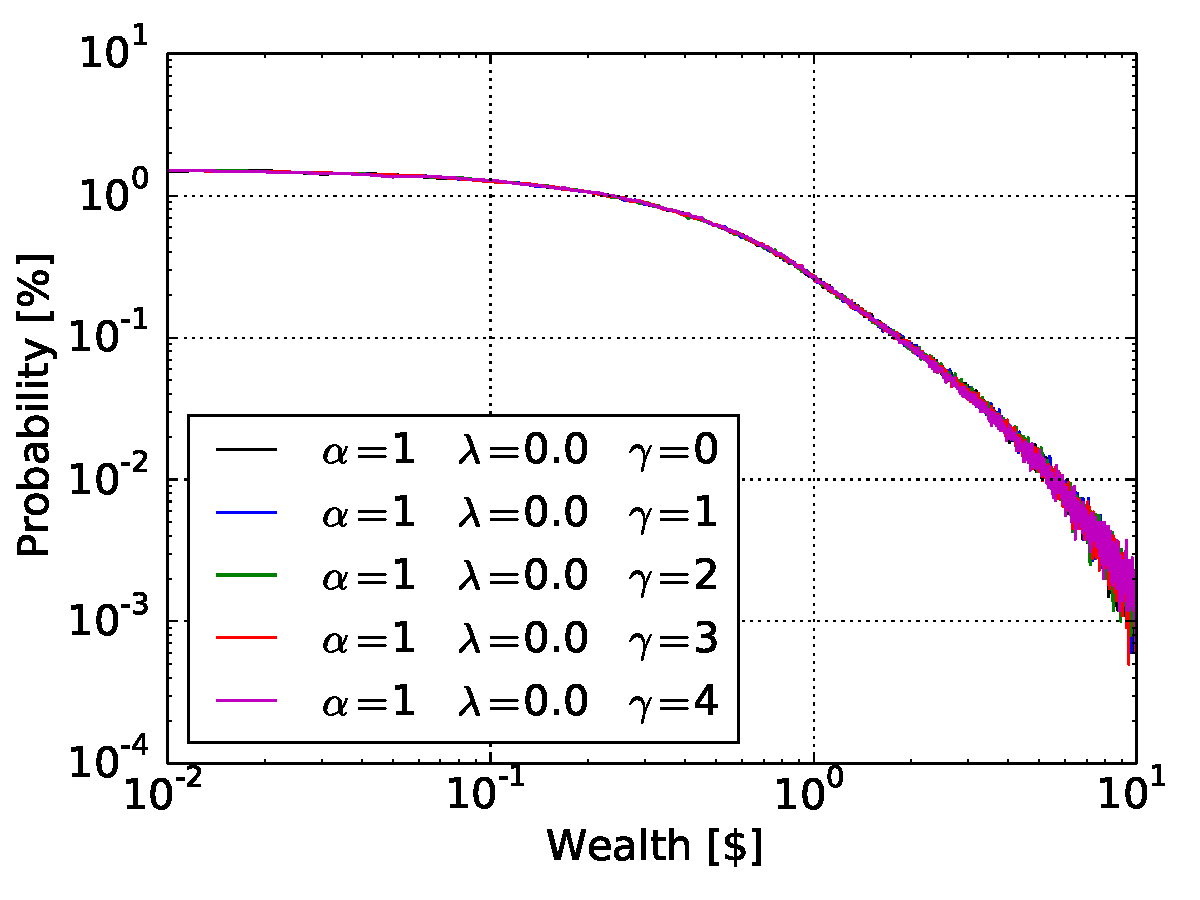
\includegraphics[width=\linewidth]{result/5e/5e-1-00-loglog}
        \caption{}
    \end{subfigure}%
    ~ 
    \begin{subfigure}{0.5\textwidth}
        \centering
        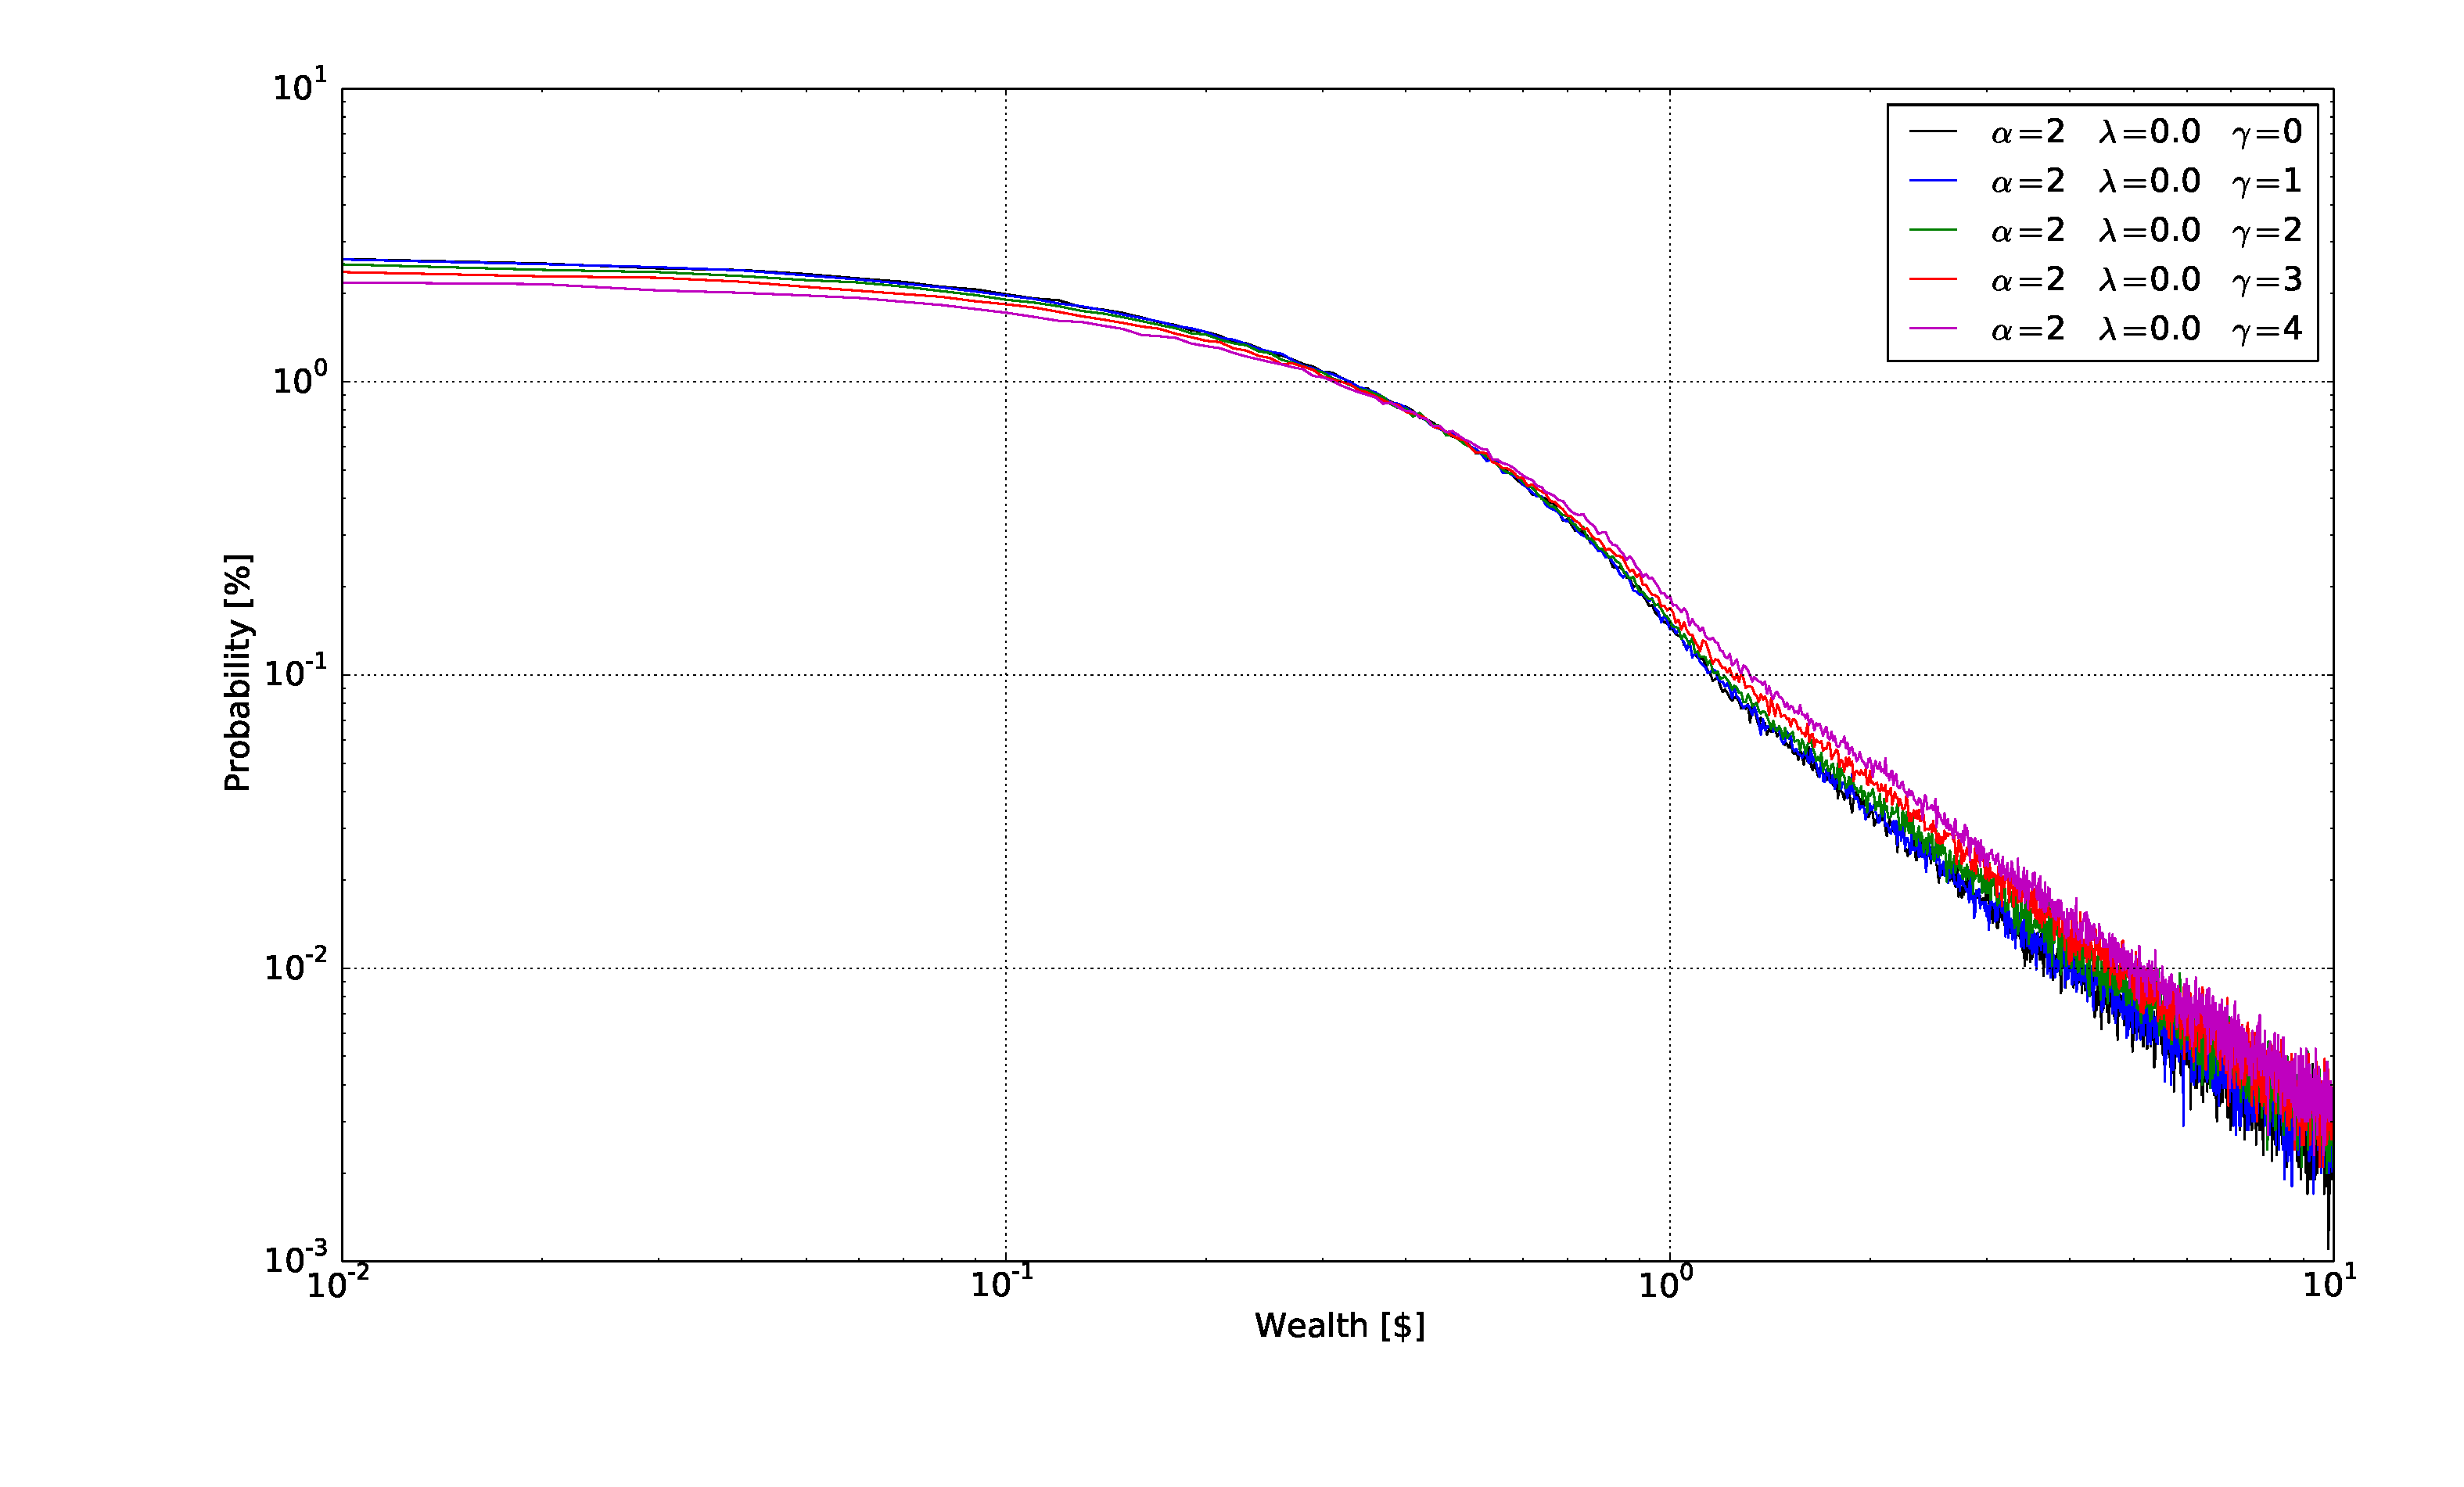
\includegraphics[width=\linewidth]{result/5e/5e-2-00-loglog}
        \caption{}
    \end{subfigure}
    \caption{logarithmic plots with no saving and four different values for $\gamma$. $\alpha$ is doubled for b) compared to a)}
    \label{fig:loglog1}
\end{figure}

The shape is recognizable from figure \ref{fig:5b} with the two values of $\alpha$. As $\alpha$ is increased we see that the effect of changing $\gamma$ is stronger, and thus has a stronger influence on the distribution. 

\begin{figure}[H]
    \centering
    \begin{subfigure}{0.5\textwidth}
        \centering
        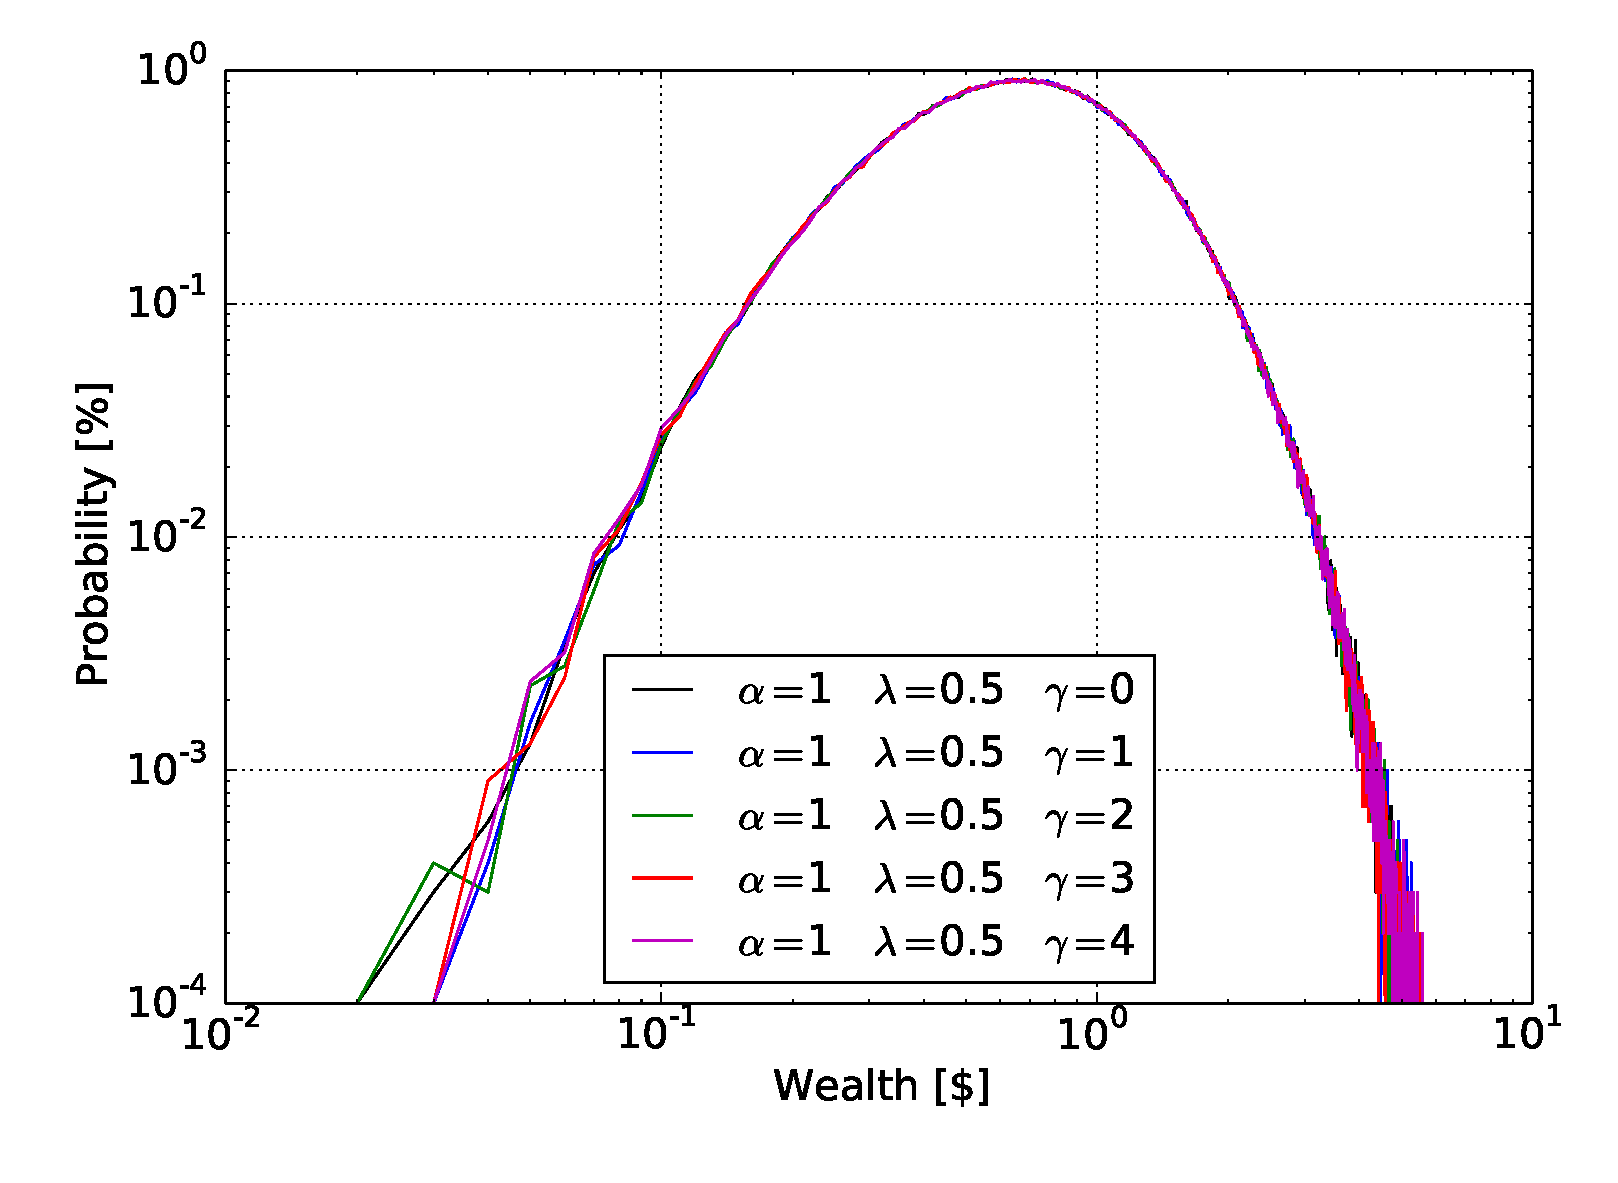
\includegraphics[width=\linewidth]{result/5e/5e-1-50-loglog}
        \caption{}
    \end{subfigure}%
    ~ 
    \begin{subfigure}{0.5\textwidth}
        \centering
        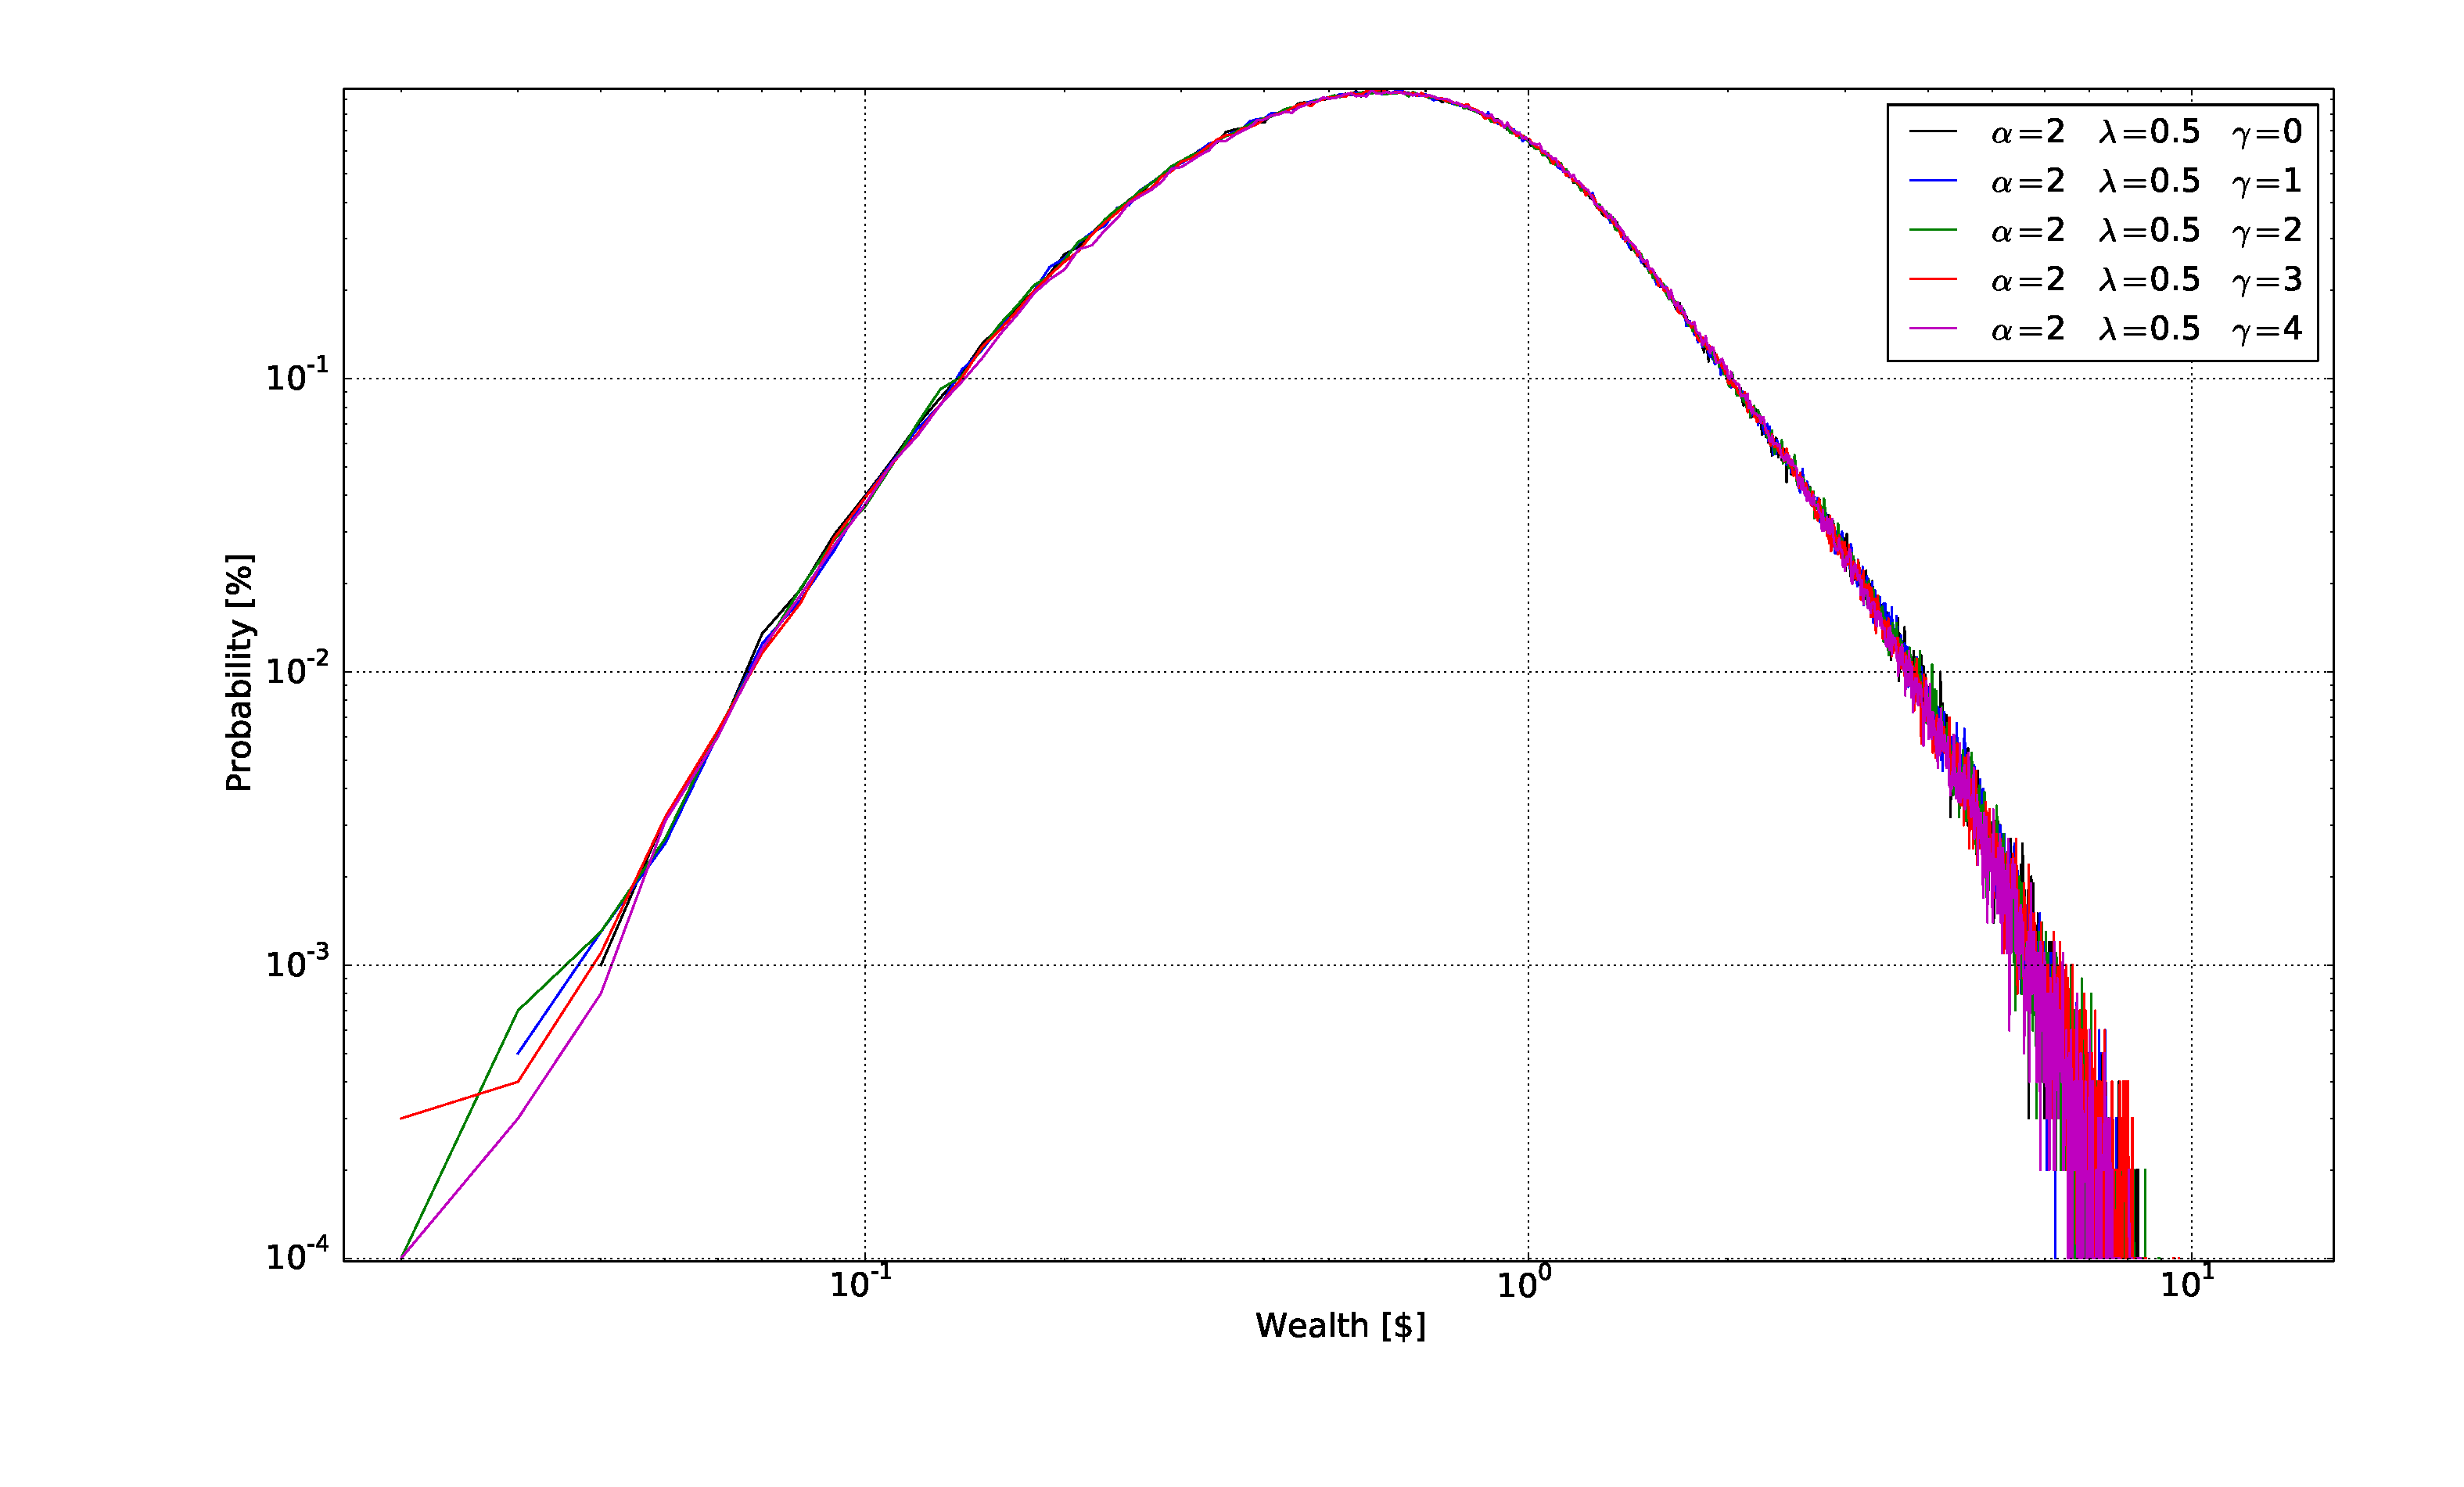
\includegraphics[width=\linewidth]{result/5e/5e-2-50-loglog}
        \caption{}
    \end{subfigure}
    \caption{plots a) and b) shows the same four distributions where there is no saving and four different values for alpha.}
    \label{fig:loglog2}
\end{figure}

When the agents are allowed to save money we again see that this effect dominates. From a technical point of view this makes sense as the savings is performed before calculating the probabilities in the simulations. $\lambda$ therefore becomes a limiting factor for the other two variables.
